\documentclass{article}

\usepackage[utf8]{inputenc}
\usepackage[T1]{fontenc}
\usepackage[francais]{babel}
\usepackage{url}
\usepackage{color}
\usepackage{verbatim}
\usepackage{amsmath,amssymb,amsfonts}
\usepackage{graphicx}
\usepackage[french]{algorithm2e}
\usepackage{geometry}
\usepackage{caption}
\captionsetup[figure]{slc=on}
\usepackage{enumitem}
\usepackage{listings}
\usepackage{listingsutf8}
\frenchbsetup{StandardLists=true}
\usepackage{mcode}
\lstset{language=matlab}
\lstset{
	breaklines=true, 
	showspaces=false, 
	keepspaces=true, 
	numbers=left, 
	frame=shadowbox, 
	keywordstyle=\color{blue},
	basicstyle=\ttfamily\small,
	commentstyle=\color{green}
}
\geometry{hmargin=2.5cm, vmargin=2.5cm}

\title{\textbf{Traitement d'images TP3 : Convolution spatiale}\\ \it{Filtrage Passe Bas : Réduction de Bruit additif} \\ \it{Filtrage Passe haut : Réhaussement de contraste}}
\author{Line \bsc{POUVARET}, Hamdi \bsc{BENAOUN}}
\date{2015-2016}

\begin{document}
\maketitle

\section*{\it{\textbf{Travail préliminaire}}}

\begin{enumerate}[label=\arabic*$\degres$)]
	\item La somme en ligne notée $s_{n}$ des éléments du triangle est égale à 2n.
	\item Par analogie avec la formule binomiale : $(x+y)^{n}=(x+y)^{n-1}*(x+y)$, on constate que $(h_{1})^{n}[k] = (h1)^{*n-1}[k]*(h_{1})[k]$

Par exemple, pour l’ordre n=2, la convolution de (1 1) avec (1 1) donne bien (1 2 1) et ainsi de suite pour les ordres supérieurs.\\

Dans MatLab : 
\begin{lstlisting}
conv2([ 1 1], [1 1]) = [1 2 1]
conv2([1 2 1], [1 1]) = [ 1 3 3 1] 
\end{lstlisting}
	\item 
Moy(n) = 0 pour chaque n.
	\begin{itemize}\renewcommand{\labelitemi}{$\bullet$}
		\item n=0 $\rightarrow$ Var(n) = 0
		\item n=1 $\rightarrow$ Var(n) = (¼)*(1/2) + (1/4)*(1/2) = 1/4
		\item n=2 $\rightarrow$ Var(n) = (1)*(1/4)+(1)*(1/4) = 1/2
		\item n=3 $\rightarrow$ Var(n) = (9/4)*(1/8)+(1/4)*(3/8) = 3/4
		\item n=4 $\rightarrow$ Var(n) = 1
		
On remarque que la Variance pour un n donné est égale à n*(1/4)
	\end{itemize}
	
\end{enumerate}

\section*{\it{\textbf{Fichier TP\_reduction\_bruit.m}}}

\begin{enumerate}[label=\arabic*$\degres$)]
	\item Dans MatLab :
	
\begin{lstlisting}
%---------------------------------------
%CALCULER LA VARIANCE DES NIVEAUX DE GRIS SUR IMA_GRIS
%variance des niveaux de gris dans l'image 
%var_ima=....... 
var_ima = var(ima_gris(:));

%FIXER LA VARIANCE DU BRUIT
%Parametrage du niveau de bruit
%rsb=..... \%en dB entre 10 et 20
%var_b= .......
rsb=10;
var_b=var_ima/(10*(rsb/10));
%----------------------
%FORMER l'IMAGE BRUITEE
%Bruit gaussien additif
%bruit= ................;
bruit=randn(size(ima_gris))*sqrt(var_b);

%Generation de l'image bruitee
%ima_bruit= ..................;
ima_bruit=ima_gris+bruit;
\end{lstlisting}



	\begin{minipage}[b]{0.40\linewidth}
		\fbox{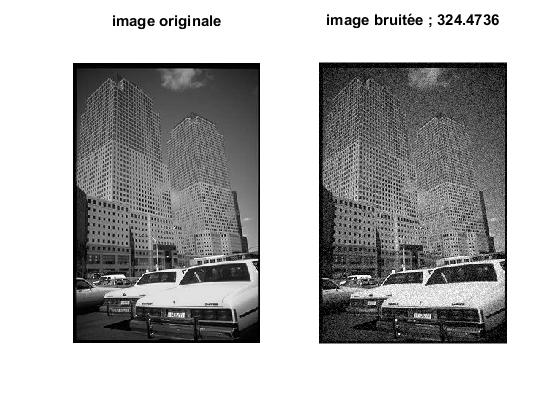
\includegraphics[width=8cm]{image_bruitee_rsb10.jpg}}
		\captionof{figure}{Image bruitée avec RSB = 10}
	\end{minipage}\hfill
	\begin{minipage}[b]{0.48\linewidth}
		\fbox{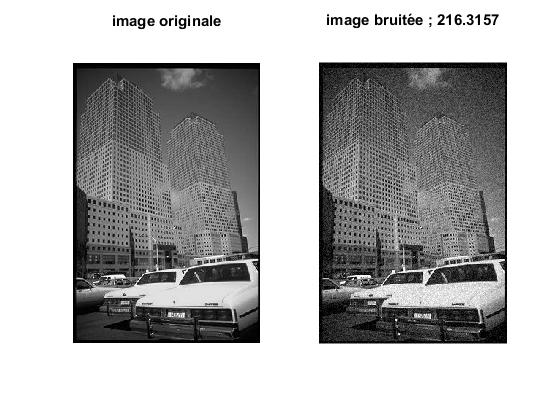
\includegraphics[width=8cm]{image_bruitee_rsb15.jpg}}
		\captionof{figure}{Image bruitée avec RSB = 15}
	\end{minipage}\hfill
	\begin{minipage}[b]{0.40\linewidth}
		\fbox{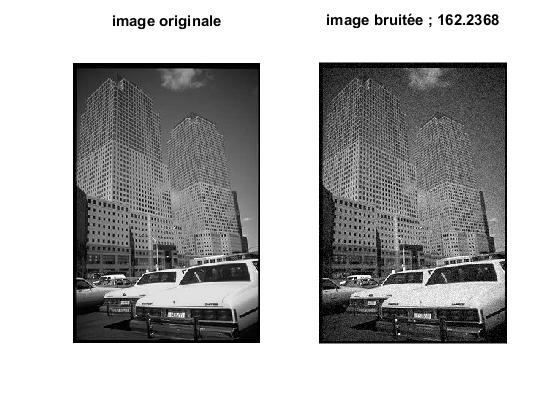
\includegraphics[width=8cm]{image_bruitee_rsb20.jpg}}
		\captionof{figure}{Image bruitée avec RSB = 20}
	\end{minipage}\hfill



On constate que plus on diminue le RSB, plus l'image sera bruitée (beaucoup plus de grains sur l'image).

	\item Dans MatLab :
\begin{lstlisting}
%Initialisation de variable si necessaire pour la generation du filtre
%binomial
%.....
for i=1:length(taille_kernel)
    
    %Convolution avec le filtre moyenne
    %-------------------------------------------------------------
    %FORMER LE NOYAU DU FILTRE MOYENNE ET EFFECTUER LA CONVOLUTION
    % kernel_moy=.........................;
    kernel_moy=ones(taille_kernel(i)).*(1/power(taille_kernel(i),2));
    % ima_moy=............................;
    ima_moy=conv2(ima_bruit,kernel_moy, 'same');
    %Convolution avec le filtre gaussien
    %----------------------------------------------------------------------
    %FORMER RECURSIVEMENT LE NOYAU DU FILTRE GAUSS ET EFFECTUER LA CONVOLUTION
    % kernel_gauss = ...........................;
    kernel_gauss = [1 1];
    for j=1:taille_kernel(i)-2
        kernel_gauss = conv2(kernel_gauss, [1 1]);
        
    end
    kernel_gauss=kernel_gauss'*kernel_gauss;
    kernel_gauss = kernel_gauss.*(1/(sum(sum(kernel_gauss))));
%Rmq : Verifier que la somme des coefficients des noyaux est egale a 1

    % ima_gauss=..........................;
    ima_gauss=conv2(ima_bruit,kernel_gauss, 'same'); 
\end{lstlisting}
    
    	\item Analyse des résultats : On considère RSB = 10 pour analyser les résultats sur une image très bruitée (différence plus notable entre les deux filtres)


\subsection*{Comparaison entre les filtres Moyenne et Gaussien pour une taille donnée de noyau}

\fbox{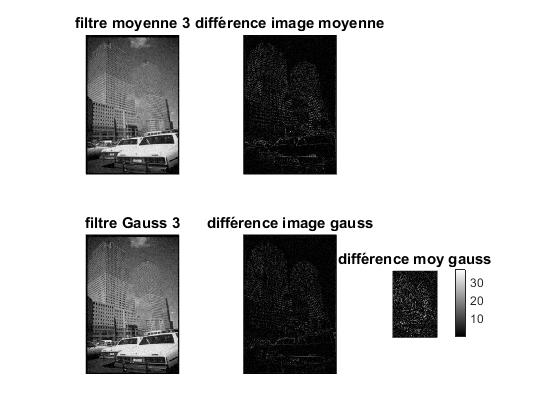
\includegraphics[width=16cm]{comp_filtre_3.jpg}}
\captionof{figure}{Moyenne VS Gaussien, K = 3}

La différence entre les deux filtres n'est pas notable pour cette taille de noyau. 

On peut à la limite voir que le filtre moyenne perd un peu les contours dans l'image par rapport au filtre gaussien.\\

Le bruit est légèrement réduit.

\fbox{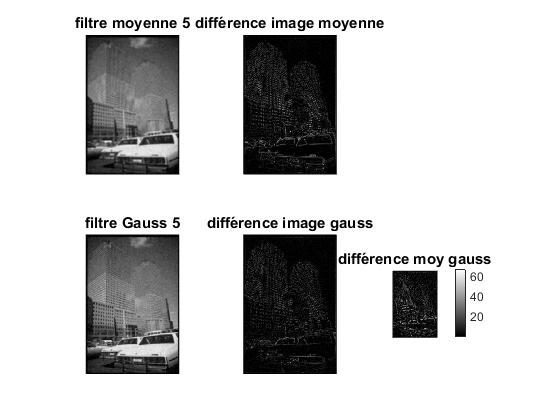
\includegraphics[width=16cm]{comp_filtre_5.jpg}}
\captionof{figure}{Moyenne VS Gaussien, K = 5}

Pour cette taille de noyau, on voit que le filtre moyenne réduit bien le bruit mais a tendance à trop flouter l'image et perdre les contours par rapport au filtre gaussien qui paraît plus efficace.\\

Le bruit est un peu plus réduit dans les deux cas.

\fbox{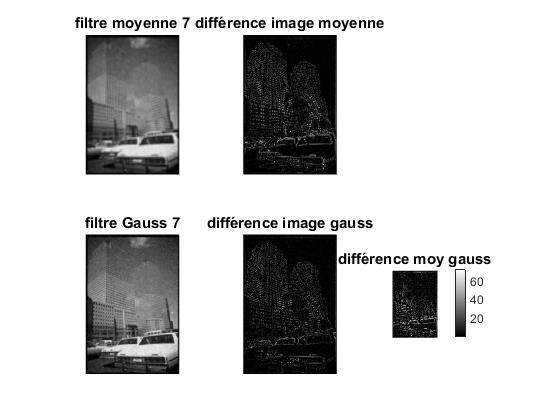
\includegraphics[width=16cm]{comp_filtre_7.jpg}}
\captionof{figure}{Moyenne VS Gaussien, K = 7}

Finalement, pour une taille de noyau de 7, le filtre moyenne floute énormément l'image, on perd quasiment tous les contours des objets et beaucoup d'information. 

Le bruit est réduit mais étant donné que l'image est très floutée, on a du mal à bien mettre en évidence la réduction du bruit.\\

Le filtre gaussien conserve beaucoup mieux les contours, les détails sont malgré tout dégradés (les fenêtres de l'immeuble par exemple) mais l'information est beaucoup mieux conservée et le bruit assez bien réduit.

\subsection*{Comparaison entre les tailles des noyaux pour chaque filtre}


\subsubsection*{Filtre moyenne}
	\begin{minipage}[b]{0.40\linewidth}
		\fbox{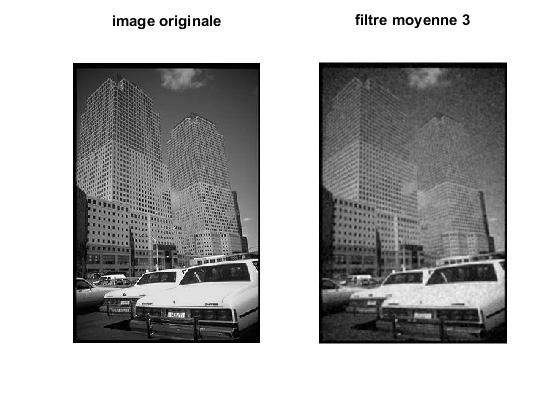
\includegraphics[width=8cm]{filtre_moy_3.jpg}}
		\captionof{figure}{Filtre moyenne, K=3}
	\end{minipage}\hfill
	\begin{minipage}[b]{0.48\linewidth}
		\fbox{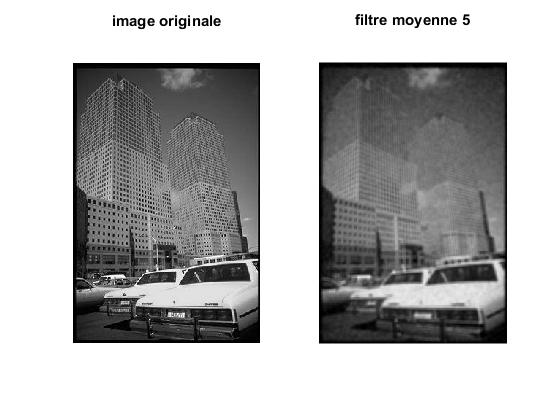
\includegraphics[width=8cm]{filtre_moy_5.jpg}}
		\captionof{figure}{Filtre moyenne, K=5}
	\end{minipage}\hfill
	\begin{minipage}[b]{0.40\linewidth}
		\fbox{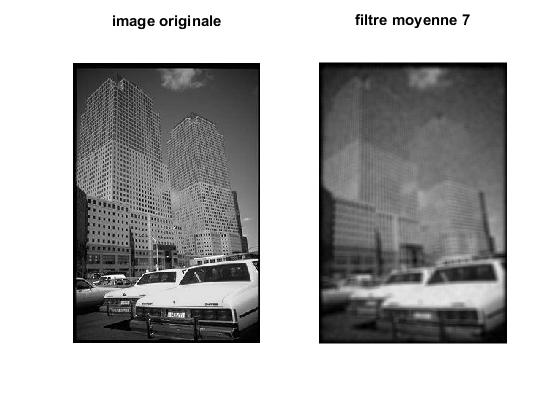
\includegraphics[width=8cm]{filtre_moy_7.jpg}}
		\caption{figure}{Filtre moyenne, K=7}
	\end{minipage}\hfill

Plus la taille du noyau de convolution va augmenter et plus l'image va se retrouver floutée avec le filtre moyenne.\\

Le bruit est de plus en plus réduit plus la taille du noyau est grande mais la perte des contours augmente aussi.


\subsubsection*{Filtre gaussien}
	\begin{minipage}[b]{0.40\linewidth}
		\fbox{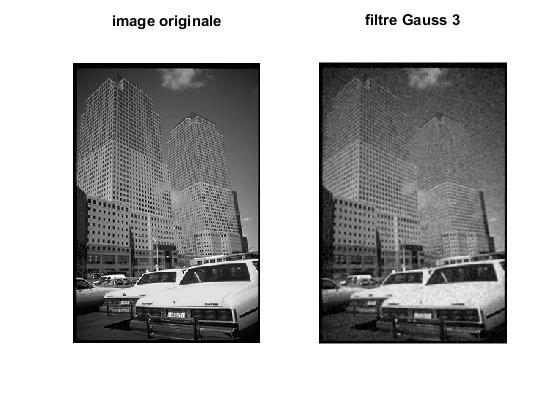
\includegraphics[width=8cm]{filtre_gauss_3.jpg}}
		\captionof{figure}{Filtre gaussien, K=3}
	\end{minipage}\hfill
	\begin{minipage}[b]{0.48\linewidth}
		\fbox{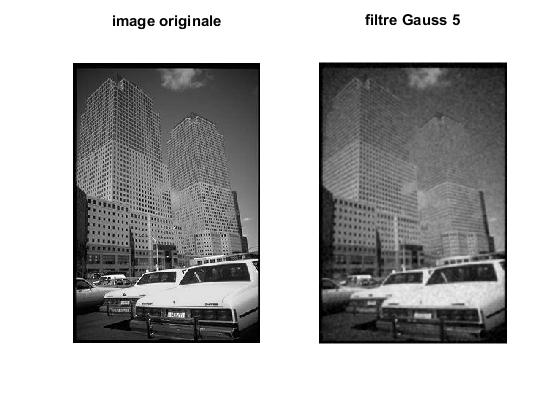
\includegraphics[width=8cm]{filtre_gauss_5.jpg}}
		\captionof{figure}{Filtre gaussien, K=5}
	\end{minipage}\hfill
	\begin{minipage}[b]{0.40\linewidth}
		\fbox{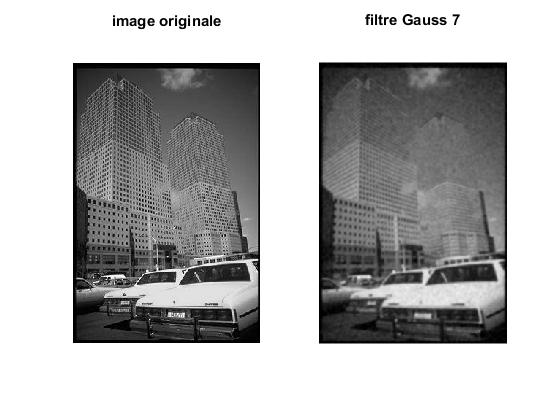
\includegraphics[width=8cm]{filtre_gauss_7.jpg}}
		\captionof{figure}{Filtre gaussien, K=7}
	\end{minipage}\hfill
	
Plus la taille du noyau de convolution va augmenter et plus le bruit va être réduit.\\

On remarque aussi que les détails les plus sombres sont de plus en plus perdus (comme les fenêtres de l'immeuble), il y a quand même un léger flou mais les contours sont globalement bien conservés.

\end{enumerate}

\section*{\it{\textbf{Fichier TP\_rehaussement.m}}}
\begin{enumerate}[label=\arabic*$\degres$)]
	\item Dans MatLab :
\begin{lstlisting}
%Filtrage Passe Haut 3 x 3
%Image filtree Passe Haut : Image originale - Image filtree Passe Bas 
%Former le noyau du filtre Passe Haut a partir de son oppose Passe Bas
%--------------- A FAIRE----------------------%
%Ker_PB = .....; 
taille_kernel = 7;
choix_filtre = 2;
if(choix_filtre == 1)
    Ker_PB = [1 1];
    for j=1:taille_kernel-2
        Ker_PB = conv2(Ker_PB, [1 1]);
    end
    Ker_PB=Ker_PB'*Ker_PB;
    Ker_PB = Ker_PB.*(1/(sum(sum(Ker_PB))));
elseif(choix_filtre == 2)
    Ker_PB=ones(taille_kernel).*(1/power(taille_kernel,2));
end
%Ker_PH = ......;
Ker_imp = zeros(taille_kernel, taille_kernel);
Ker_imp((taille_kernel+1)/2, (taille_kernel+1)/2) = 1;
Ker_PH = Ker_imp - Ker_PB;
\end{lstlisting}
\begin{lstlisting}
%Filtrage Passe Haut de rehaussement 
%Image rehaussee = image originale + alpha * image filtree passe haut
%Former le noyau de convolution du filtre equivalent
%alpha = ... ; 
%Ker_RH = ..... ; 
alpha = 1/9;
Ker_RH = Ker_imp + alpha*Ker_PH;
\end{lstlisting}

	\item Variations...
\end{enumerate}

\end{document}